% IEEE-style two-column report. NOTE: the official IEEEtran.cls was not available in the build environment, so this uses
% article+twocolumn with IEEE-like settings. To use the official class: replace the preamble up to \begin{document} by
% \documentclass[conference]{IEEEtran} and the title block by \IEEEauthorblockN/\IEEEauthorblockA.
\documentclass[10pt,twocolumn,letterpaper]{article}
\usepackage[top=0.75in,bottom=1in,left=0.625in,right=0.625in,columnsep=0.25in]{geometry}
\usepackage{mathptmx}
\usepackage[T1]{fontenc}
\usepackage{amsmath,amssymb,booktabs,graphicx,url,cite,balance}
\usepackage[labelsep=period,font=small]{caption}
\usepackage[compact]{titlesec}
\titleformat{\section}{\centering\normalfont\small\scshape}{\Roman{section}.}{0.5em}{}
\titleformat{\subsection}{\normalfont\small\itshape}{\Alph{subsection}.}{0.5em}{}
\titlespacing*{\section}{0pt}{8pt}{3pt}\titlespacing*{\subsection}{0pt}{5pt}{2pt}
\setlength{\parindent}{1em}\setlength{\parskip}{0pt}
\renewcommand{\arraystretch}{0.95}\setlength{\tabcolsep}{3pt}
\captionsetup[table]{labelfont=sc,textfont=sc,skip=3pt}
\newcommand{\silu}{\mathrm{silu}}
\begin{document}
\title{\vspace{-0.4in}\LARGE Kolmogorov--Arnold Networks: From-Scratch Implementation, Reduced-Scale Reproduction and Ablations\vspace{-0.1in}}
\author{\small Dhruv (Roll No.\ 24CS3018)\\[-1pt]\small Dept.\ of Computer Science and Engineering, Rajiv Gandhi Institute of Petroleum Technology (RGIPT)\\[-1pt]\small \texttt{24cs3018@rgipt.ac.in}}
\date{}
\maketitle\vspace{-0.3in}

\begin{abstract}
We re-implement Kolmogorov--Arnold Networks (KANs) \cite{liu2025kan} from scratch in PyTorch: Cox--de Boor B-splines, the residual spline edge function, KAN layers, on-the-fly grid update and least-squares \emph{grid extension}, plus sparsification, pruning and symbolic simplification. At reduced scale we reproduce the central qualitative findings on $f(x,y)=\exp(\sin\pi x+y^2)$: staircase loss curves under grid extension, power-law decay of test error with grid size, and a KAN with 315 parameters (test RMSE $1.8\times10^{-5}$) beating parameter-matched MLPs by about 60$\times$ (best MLP, 501 parameters: $1.2\times10^{-3}$). The result is fragile, however: only one of four seeds reaches this regime and the median KAN is worse than the best MLP. Two ablations show that grid extension helps at large $G$ but not at small $G$, and that higher spline order lowers the error. Extensions to Feynman symbolic regression, a Poisson PDE and MNIST give a mixed picture (single seed each): the KAN beats an equal-parameter MLP on three of six Feynman equations and on the PDE only modestly and only at the largest size, loses on MNIST (92--94\% vs.\ 97\%), and automatic symbolic simplification did not recover any of the target formulas (Sec.~\ref{sec:ext}).
\end{abstract}
\par\vspace{2pt}\noindent\textit{Index Terms}---Kolmogorov--Arnold networks, B-splines, grid extension, neural scaling laws, symbolic regression.

\section{Introduction}
Multilayer perceptrons (MLPs) place fixed activations on nodes and learn linear weights on edges. KANs \cite{liu2025kan} invert this: every edge carries a learnable univariate function, parametrised as a B-spline \cite{deboor1978}, and nodes only sum their inputs. Motivated by the Kolmogorov--Arnold representation theorem, the paper claims faster neural scaling laws and interpretability on small, smooth, compositional problems. This project (i) implements the defining components without any KAN library, (ii) reproduces the paper's Fig.~2.3 / Sec.~2.4 and the $\exp(\sin\pi x+y^2)$ panel of Fig.~3.1 at reduced scale, (iii) tests two design choices by ablation, and (iv) adds the simplification pipeline and equal-parameter comparisons required by the assignment. We state wherever our numbers disagree with the paper.

\section{Method}
\subsection{KAN layer and network}
A layer with $n_{in}$ inputs and $n_{out}$ outputs holds a matrix of univariate functions, and nodes only sum: $x_{l+1,j}=\sum_i\phi_{l,j,i}(x_{l,i})$ (paper Eq.~2.5--2.7). Each edge is
\begin{equation}
\phi(x)=w_b\,\silu(x)+w_s\sum_{i=1}^{G+k}c_i B_i(x),
\end{equation}
with trainable $w_b,w_s,c_i$ (Eq.~2.10--2.12), initialised as in the paper ($c_i\!\sim\!\mathcal N(0,0.1^2)$, $w_s=1$, Xavier $w_b$). The $B_i$ are order-$k$ B-splines on a grid of $G$ intervals computed by the Cox--de Boor recursion; they were checked against SciPy in the unit tests. A KAN of shape $[n_0,\dots,n_L]$ has $\mathcal O(N^2L(G+k))$ parameters; e.g.\ $[2,1,1]$ has $3(G+k+2)$, i.e.\ 24 at $G{=}3$ and 315 at $G{=}100$ for $k{=}3$.

\subsection{Grid update and grid extension}
Grids are re-placed on the fly from the data seen by each edge. Our knot rule (unspecified in the paper) mixes uniform and quantile knots, adds a 1\% margin and fixes the outer knots at the margin edges. \emph{Grid extension} (Eq.~2.16) refits a finer spline on $G'$ intervals to the current coarse one by least squares, $\min_{c'}\mathbb E_x\big|\sum_j c'_jB'_j(x)-\sum_i c_iB_i(x)\big|^2$, so the function is preserved while resolution increases.

\subsection{Sparsification, pruning, symbolification}
With $|\phi|_1$ the mean absolute value of an edge over the training inputs, a layer's norm is $|\Phi|_1=\sum_{ij}|\phi_{ij}|_1$ and its entropy $S(\Phi)=-\sum_{ij}\frac{|\phi_{ij}|_1}{|\Phi|_1}\log\frac{|\phi_{ij}|_1}{|\Phi|_1}$. Training minimises $\ell_{pred}+\lambda\sum_l(|\Phi_l|_1+S(\Phi_l))$ (Eq.~2.17--2.20). Hidden nodes whose incoming or outgoing maximal edge norm is below $\theta{=}10^{-2}$ are pruned (Eq.~2.21). Each surviving edge is then matched to a library function ($x,x^2,x^3,x^4,1/x,\sqrt x,|x|,e^x,\ln x,\sin,\cos,\tanh$) by fitting $y\approx c\,f(ax{+}b)+d$ (grid search over $(a,b)$, closed-form $(c,d)$, scored by $R^2$, simplest function among ties); the affine parameters are fine-tuned and a SymPy expression is composed from the edges.

\section{Experimental setup}
\textbf{Task.} $f(x,y)=\exp(\sin\pi x+y^2)$ with $x,y\sim U[-1,1]$ (domain unspecified in the paper); 1000 training, 1000 validation and 10\,000 test points from independent random streams, float64, no preprocessing. \textbf{Models.} KAN $[2,1,1]$ (4 seeds) and $[2,5,1]$ (2 seeds), $k{=}3$, $G\in\{3,5,10,20,50,100\}$ with grid extension and 100 LBFGS steps per grid (the paper uses 200 steps and $G$ up to 1000); MLPs with SiLU, depth 2--4, widths 5--50, 4 seeds each and 600 steps (equal to the KAN's total). A step is one \texttt{LBFGS.step} with strong-Wolfe line search and \texttt{max\_iter}=20. \textbf{Selection.} Seeds, checkpoints and MLP configurations are chosen on \emph{validation} RMSE only; test RMSE is only reported. \textbf{Metrics.} Test RMSE, $\sqrt{\mathrm{median}(\text{sq.\ err.})}$, the log--log slope $\alpha$ against $G$, parameter count and seconds. Everything was run on a single CPU thread; all tables and figures are generated from saved CSV files. \textbf{Implementation checks.} 20 unit tests pass (B-spline partition of unity and SciPy agreement, extension preserves the function, regulariser, pruning, symbolic fit, matched-MLP counts, PDE residual).

\section{Results: reproduction}
\subsection{Grid extension and scaling}
Fig.~\ref{fig:stair} shows the staircase loss: each extension drops the error and training then plateaus. Table~\ref{tab:grid} and Fig.~\ref{fig:scale} give test error against $G$. For the validation-selected seed the test RMSE falls from $1.7\times10^{-2}$ at $G{=}3$ to $4.7\times10^{-5}$ at $G{=}20$ (slope $\alpha=3.15$ on $G\le20$, a window chosen after seeing the curve; $3.29$ for $\sqrt{\mathrm{median}}$), then saturates at $1.8\times10^{-5}$ at $G{=}100$, so the slope over the whole range is only $2.02$ ($2.45$ for the median-based error). The paper reports $\approx3$ and, for the median error, closer to the theoretical 4. We therefore reproduce the power-law regime at small $G$ but \emph{not} the slope close to 4 or the extent of the scaling range; a modest generalisation gap appears at large $G$ (train $8.5\times10^{-6}$ vs.\ test $1.8\times10^{-5}$ at $G{=}100$).

\textbf{Seed sensitivity.} LBFGS lands in different local minima: at $G{=}100$ three of four seeds are below $10^{-2}$, but only one reaches $\sim\!10^{-5}$; the others end at $2.3\times10^{-3}$, $4.4\times10^{-3}$ and $0.46$ (median $3.4\times10^{-3}$). Results also depend on the CPU thread count (1 vs.\ 2 threads gave $2.69\times10^{-2}$ vs.\ $2.71\times10^{-2}$ at $G{=}3$ and $3.4\times10^{-3}$ vs.\ $4.6\times10^{-3}$ at $G{=}10$ for seed~0), so individual numbers are not bit-reproducible.

\textbf{Wide network.} For $[2,5,1]$ the validation-optimal grid is $G{=}20$ for both seeds (test RMSE $1.3\times10^{-4}$ and $4.5\times10^{-4}$), whereas the paper observes the interpolation threshold near $G{\approx}50$ (predicted $\approx67$). The wide network is far more consistent across seeds but its best error is higher than the best $[2,1,1]$ seed.

\subsection{KAN versus MLP at equal parameters}
Table~\ref{tab:mlp} and Fig.~\ref{fig:mlp} compare the validation-selected KAN seed with the best-of-4 MLP at the closest parameter counts. The KAN is better at every size, by a factor of about 6 to 500 (largest at mid sizes): e.g.\ $3.7\times10^{-4}$ (45 parameters) vs.\ $5.2\times10^{-3}$ (51), and $1.8\times10^{-5}$ (315) vs.\ $1.2\times10^{-3}$ for the best MLP (501 parameters), a factor $\approx64$, while MLP errors flatten as the paper reports. This is a best-seed comparison on both sides; the \emph{median} KAN ($3.4\times10^{-3}$ at 315 parameters) is worse than the best MLP ($1.4\times10^{-3}$ at 261), so the advantage depends on being able to try several seeds. The KAN is also slower: a full six-stage KAN run took 127--161\,s against 19--28\,s for a 600-step MLP on our single CPU thread.

\subsection{What the KAN learned}
For a $[2,1,1]$ KAN from a separate live run (test RMSE $3.0\times10^{-5}$) the first-layer edges recover $\sin\pi x$ and $y^2$ up to affine maps (absolute correlation 1.000 on a dense grid) and the second-layer edge is exponential-like (Fig.~\ref{fig:edges}), i.e.\ the compositional structure of $f$ is read directly from the splines.

\begin{figure}[t]\centering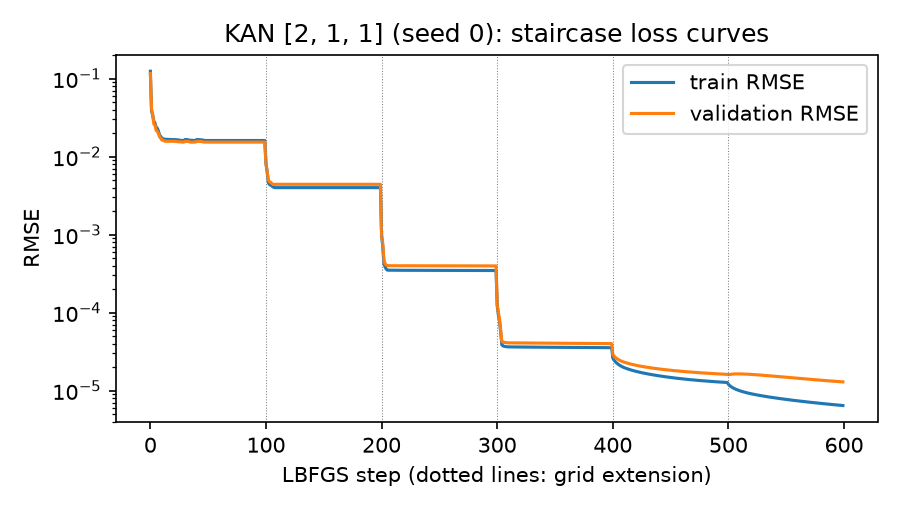
\includegraphics[width=0.93\columnwidth]{../figures/live_training_curves.png}
\caption{Staircase loss of a $[2,1,1]$ KAN (live run): dotted lines mark the extensions to $G=5,10,20,50,100$ (100 steps each).}\label{fig:stair}\end{figure}
\begin{figure*}[t]\centering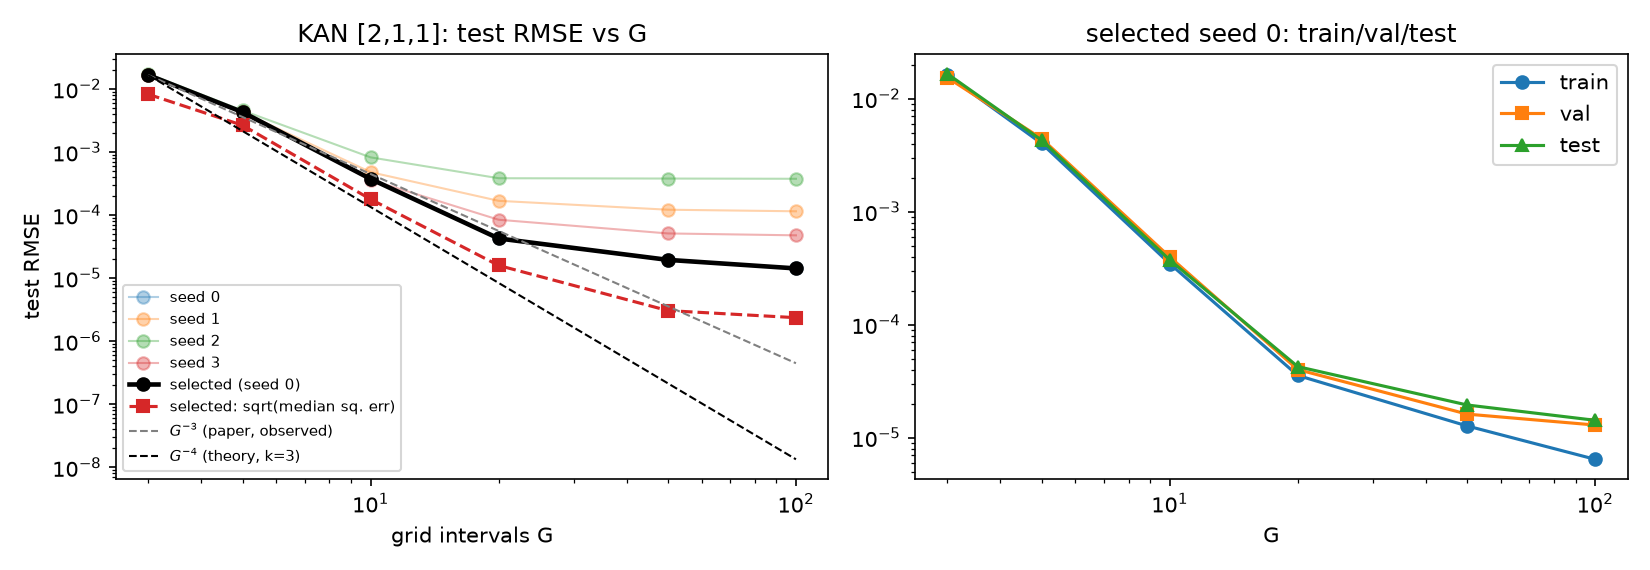
\includegraphics[width=0.84\textwidth]{../figures/scaling_vs_G.png}
\caption{Left: test RMSE vs.\ $G$ for four seeds (faded), the validation-selected seed (bold), its median-based error, and the $G^{-3}$ and $G^{-4}$ references. Right: train/validation/test RMSE of the selected seed.}\label{fig:scale}\end{figure*}
\begin{figure*}[t]\centering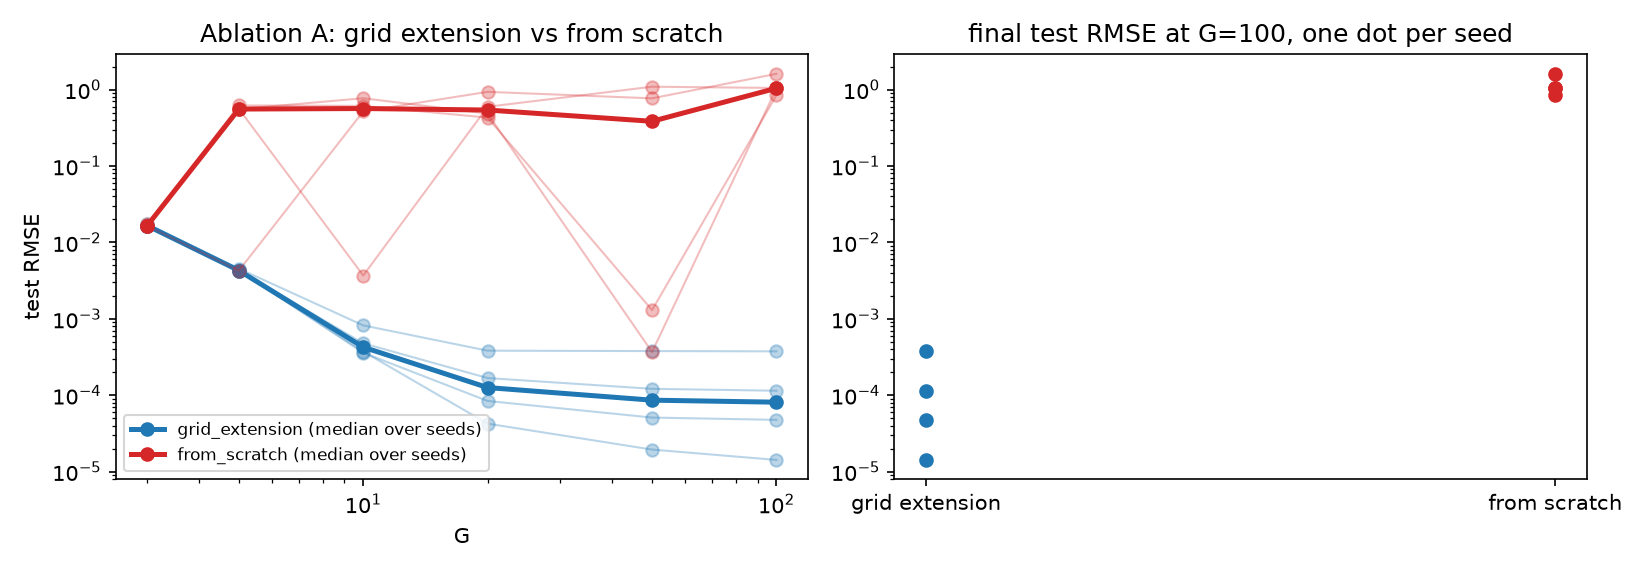
\includegraphics[width=0.84\textwidth]{../figures/ablation_extension.png}
\caption{Ablation A. Left: test RMSE vs.\ $G$ (faded: individual seeds). Right: final test RMSE at $G{=}100$.}\label{fig:ablA}\end{figure*}
\begin{table}[t]
\caption{KAN [2,1,1], $k{=}3$. Selected seed (3) chosen on final validation RMSE; median and success count (test RMSE $<10^{-2}$) are over 4 seeds.}\label{tab:grid}
\centering\footnotesize
\begin{tabular}{rrrrrrr}
\toprule
$G$ & params & train & val & test (sel.) & test (median) & seeds ok \\
\midrule
3 & 24 & $1.6\!\times\!10^{-2}$ & $1.5\!\times\!10^{-2}$ & $1.7\!\times\!10^{-2}$ & $3.4\!\times\!10^{-1}$ & 0/4 \\
5 & 30 & $4.0\!\times\!10^{-3}$ & $4.4\!\times\!10^{-3}$ & $4.3\!\times\!10^{-3}$ & $3.1\!\times\!10^{-1}$ & 1/4 \\
10 & 45 & $3.4\!\times\!10^{-4}$ & $3.9\!\times\!10^{-4}$ & $3.7\!\times\!10^{-4}$ & $2.7\!\times\!10^{-2}$ & 2/4 \\
20 & 75 & $4.0\!\times\!10^{-5}$ & $4.4\!\times\!10^{-5}$ & $4.7\!\times\!10^{-5}$ & $5.9\!\times\!10^{-3}$ & 3/4 \\
50 & 165 & $1.6\!\times\!10^{-5}$ & $2.0\!\times\!10^{-5}$ & $2.4\!\times\!10^{-5}$ & $3.3\!\times\!10^{-3}$ & 3/4 \\
100 & 315 & $8.5\!\times\!10^{-6}$ & $1.5\!\times\!10^{-5}$ & $1.8\!\times\!10^{-5}$ & $3.4\!\times\!10^{-3}$ & 3/4 \\
\bottomrule
\end{tabular}
\end{table}

\begin{table}[t]
\caption{Equal-parameter comparison (test RMSE). MLP: best of 4 seeds by validation, 600 LBFGS steps; KAN: selected seed, grid with the closest parameter count, and median over seeds.}\label{tab:mlp}
\centering\footnotesize
\begin{tabular}{lrrrrr}
\toprule
MLP & params & test & KAN params (G) & test (sel.) & test (median) \\
\midrule
depth 2, w=5 & 21 & $1.1\!\times\!10^{-1}$ & 24 (G=3) & $1.7\!\times\!10^{-2}$ & $3.4\!\times\!10^{-1}$ \\
depth 2, w=10 & 41 & $4.3\!\times\!10^{-2}$ & 45 (G=10) & $3.7\!\times\!10^{-4}$ & $2.7\!\times\!10^{-2}$ \\
depth 3, w=5 & 51 & $5.2\!\times\!10^{-3}$ & 45 (G=10) & $3.7\!\times\!10^{-4}$ & $2.7\!\times\!10^{-2}$ \\
depth 2, w=20 & 81 & $1.8\!\times\!10^{-2}$ & 75 (G=20) & $4.7\!\times\!10^{-5}$ & $5.9\!\times\!10^{-3}$ \\
depth 4, w=5 & 81 & $2.1\!\times\!10^{-3}$ & 75 (G=20) & $4.7\!\times\!10^{-5}$ & $5.9\!\times\!10^{-3}$ \\
depth 3, w=10 & 151 & $1.8\!\times\!10^{-3}$ & 165 (G=50) & $2.4\!\times\!10^{-5}$ & $3.3\!\times\!10^{-3}$ \\
depth 2, w=50 & 201 & $1.3\!\times\!10^{-2}$ & 165 (G=50) & $2.4\!\times\!10^{-5}$ & $3.3\!\times\!10^{-3}$ \\
depth 4, w=10 & 261 & $1.4\!\times\!10^{-3}$ & 315 (G=100) & $1.8\!\times\!10^{-5}$ & $3.4\!\times\!10^{-3}$ \\
depth 3, w=20 & 501 & $1.2\!\times\!10^{-3}$ & 315 (G=100) & $1.8\!\times\!10^{-5}$ & $3.4\!\times\!10^{-3}$ \\
\bottomrule
\end{tabular}
\end{table}

\begin{table}[t]
\caption{Ablation A, test RMSE over seeds: grid extension vs re-initialising at every $G$ (same steps, data, seeds).}\label{tab:ablA}
\centering\footnotesize
\begin{tabular}{rrrrrrr}
\toprule
$G$ & ext.\ best & ext.\ median & ok & scratch best & scratch median & ok \\
\midrule
3 & $1.7\!\times\!10^{-2}$ & $3.4\!\times\!10^{-1}$ & 0/4 & $1.7\!\times\!10^{-2}$ & $3.4\!\times\!10^{-1}$ & 0/4 \\
5 & $4.3\!\times\!10^{-3}$ & $3.1\!\times\!10^{-1}$ & 1/4 & $4.3\!\times\!10^{-3}$ & $4.4\!\times\!10^{-3}$ & 3/4 \\
10 & $3.7\!\times\!10^{-4}$ & $2.7\!\times\!10^{-2}$ & 2/4 & $3.6\!\times\!10^{-4}$ & $4.1\!\times\!10^{-4}$ & 4/4 \\
20 & $4.7\!\times\!10^{-5}$ & $5.9\!\times\!10^{-3}$ & 3/4 & $1.0\!\times\!10^{-4}$ & $4.9\!\times\!10^{-1}$ & 1/4 \\
50 & $2.4\!\times\!10^{-5}$ & $3.3\!\times\!10^{-3}$ & 3/4 & $1.6\!\times\!10^{-4}$ & $5.4\!\times\!10^{-1}$ & 1/4 \\
100 & $1.8\!\times\!10^{-5}$ & $3.4\!\times\!10^{-3}$ & 3/4 & $9.3\!\times\!10^{-1}$ & $1.0\!\times\!10^{0}$ & 0/4 \\
\bottomrule
\end{tabular}
\end{table}

\begin{table}[t]
\caption{Ablation B: spline order. $\alpha$ is the log--log slope of test RMSE vs.\ $G$ for the validation-selected seed up to the validation-optimal $G^\star$.}\label{tab:ablB}
\centering\footnotesize
\begin{tabular}{lrrrrr}
\toprule
order & $\alpha$ & $k{+}1$ & $G^\star$ & best test & seeds ok \\
\midrule
k=1 & 1.86 & 2 & 50 & $9.8\!\times\!10^{-4}$ & 3/4 \\
k=2 & 2.31 & 3 & 50 & $1.4\!\times\!10^{-4}$ & 1/4 \\
k=3 & 2.46 & 4 & 50 & $2.4\!\times\!10^{-5}$ & 3/4 \\
\bottomrule
\end{tabular}
\end{table}

\begin{figure}[t]\centering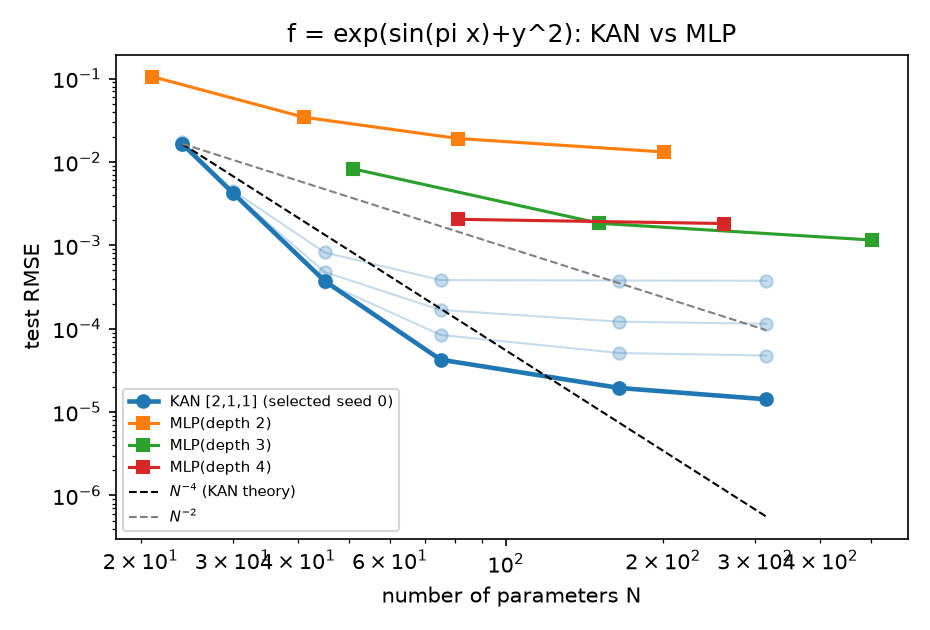
\includegraphics[width=0.95\columnwidth]{../figures/kan_vs_mlp.png}
\caption{Test RMSE vs.\ parameters: KAN seeds (faded), selected KAN, and MLPs of depth 2--4.}\label{fig:mlp}\end{figure}
\begin{figure}[t]\centering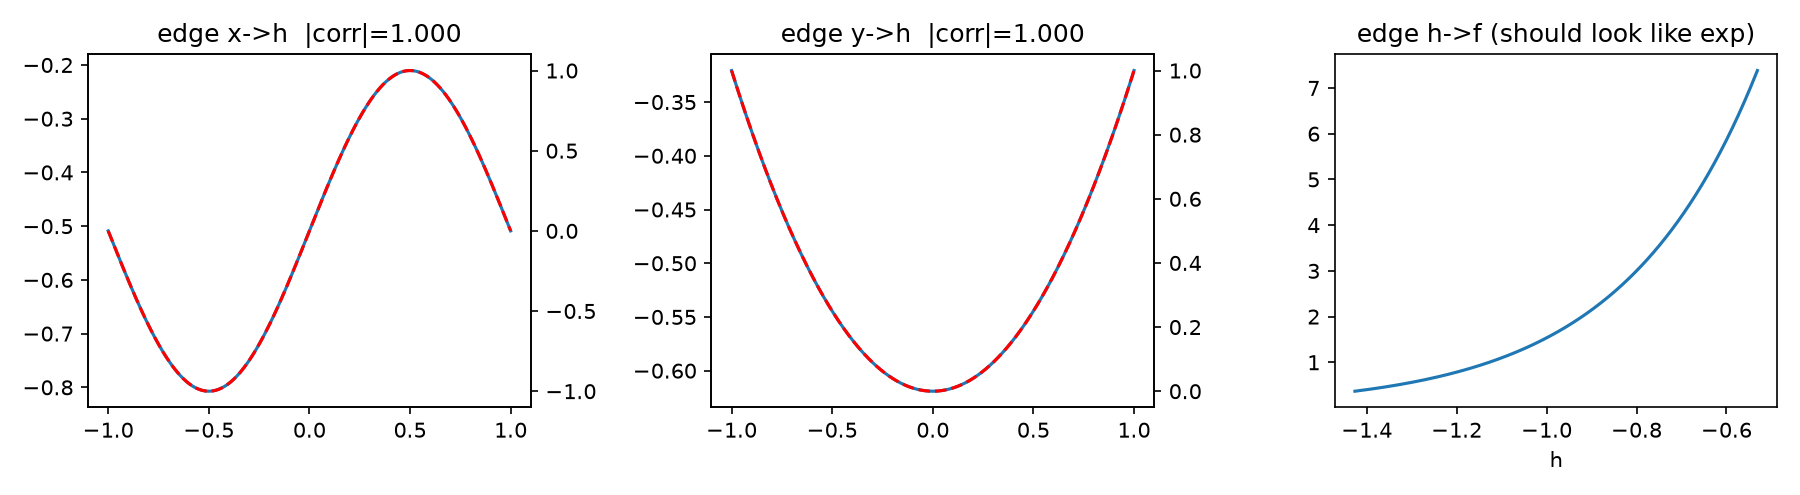
\includegraphics[width=\columnwidth]{../figures/learned_edges.png}
\caption{Learned edges (dashed red: $\sin\pi x$ and $y^2$ on twin axes).}\label{fig:edges}\end{figure}

\section{Results: ablations}
\textbf{A. Grid extension vs.\ training from scratch.} \emph{Hypothesis:} extension reaches lower error than re-initialising a KAN at each $G$ with the same budget. Table~\ref{tab:ablA} and Fig.~\ref{fig:ablA} show that this holds only for large grids: at $G\ge20$ extension reaches $<10^{-2}$ on 3 of 4 seeds, from scratch on 1 of 4 at $G{=}20$ and~50 and on none at $G{=}100$ (errors $\approx1$). At small $G$ the picture reverses: at $G{=}5$ and 10 from-scratch succeeds on 3/4 and 4/4 seeds versus 1/4 and 2/4 for extension, because a seed that fails at $G{=}3$ passes its failure down the chain whereas a re-initialised model gets a fresh start. At $G{=}20$ the best from-scratch run ($1.0\times10^{-4}$) is worse than the best extended run ($4.7\times10^{-5}$). Our hypothesis ``extension is better at every $G$'' is therefore \emph{not} supported; extension is what makes large grids trainable at all. With four seeds these counts are indicative only.

\textbf{B. Spline order.} \emph{Hypothesis:} the error decays faster in $G$ for higher $k$ (theory: $\alpha\approx k{+}1$). Table~\ref{tab:ablB} gives slopes $1.86/2.31/2.46$ for $k=1/2/3$ (theory $2/3/4$) up to $G^\star{=}50$, and best test errors $9.8\times10^{-4}$, $1.4\times10^{-4}$ and $2.4\times10^{-5}$ at $G{=}50$. The ordering is as predicted, while the slopes fall below $k{+}1$ for $k\ge2$ (optimisation and boundary effects). Only 1/4 seeds is below $10^{-2}$ at $G{=}50$ for $k{=}2$ against 3/4 for $k{=}1,3$, so this ablation also reflects seed luck.


\section{Extensions: simplification, PDE and MNIST}\label{sec:ext}
These parts were run once by the author (a single seed and a single configuration each, in the accompanying notebook) and Tables~\ref{tab:feyn}--\ref{tab:mnist} are generated from the saved CSV files. They are small-scale studies without error bars, so differences of a factor $<2$ should not be over-read.

\subsection{Feynman equations and symbolic simplification}
Six two-variable equations from the paper's Table~2 (I.6.2, I.12.11, I.16.6, I.27.6, I.44.4, II.35.18) with our own sampling ranges (2000/1000/5000 train/val/test points; the paper's numbers are therefore not comparable). For each we train (i) a human-constructed KAN with the paper's shape and grid extension $G\in\{3,5,10\}$ (100 steps each), (ii) an MLP with the same parameter count (depth 2--4 chosen on validation, 300 LBFGS steps), (iii) a $[n,5,1]$ KAN trained with sparsification ($\lambda{=}0.01$, best of 2 seeds on validation), pruned with $\theta{=}10^{-2}$ and compared with an MLP of the pruned size, and (iv) the symbolic formula obtained from the pruned KAN.

\textbf{Human-constructed KAN vs.\ MLP (Table~\ref{tab:feyn}).} The KAN is better on three equations (I.12.11 by $6.7\times$, I.27.6 by $4.3\times$, I.44.4 by $26\times$), tied on I.16.6 ($4.2\times10^{-3}$ for both) and clearly worse on I.6.2 ($20\times$) and II.35.18 ($41\times$). So the equal-parameter advantage seen in Part~A is not general; this mixed outcome is in the spirit of the paper's Table~2, where the MLP also wins on several equations.

\textbf{Pruned KAN.} Sparsification plus pruning shrank every network (e.g.\ 105 to 30 parameters for I.6.2, 45 to 30 for II.35.18), but the pruned KAN was worse than its size-matched MLP on five of six equations (better only on I.16.6, $2.2\times10^{-2}$ vs.\ $4.7\times10^{-2}$) and worse than the unpruned human KAN on all six (II.35.18 essentially equal). We did not tune $\lambda$, the shape or the number of steps as the paper does.

\textbf{Symbolic formulas.} The symbolic test RMSE ranges from $2.6\times10^{-3}$ (I.27.6) to $1.5\times10^{-1}$ (I.16.6) and is in every case at least as large as the pruned KAN's error; none approaches the machine-precision regime that signals an exact formula, and the extracted expressions are not the target forms (for I.27.6, $1/(1{+}ab)$, the pipeline returned a cubic of logarithms with RMSE $2.6\times10^{-3}$). Plausible causes, which we did not test, are the greedy best-$R^2$ choice per edge (products and ratios need compositions such as $ab=((a{+}b)^2-(a{-}b)^2)/4$ that the paper builds by hand), only one $\lambda$ and two seeds, and too few fine-tuning steps. We therefore do \emph{not} claim that our simplification pipeline recovers symbolic laws on these tasks; its components (regulariser, pruning, affine fitting) are unit-tested, but end-to-end success on the Feynman set is not demonstrated here.

\subsection{Poisson PDE}
$u_{xx}+u_{yy}=f$ on $[-1,1]^2$, $u|_{\partial\Omega}=0$, exact solution $\sin(\pi x)\sin(\pi y^2)$. The loss is $\alpha\,\mathrm{mean}|u_{xx}{+}u_{yy}{-}f|^2+\mathrm{mean}\,u_b^2$ with $\alpha{=}0.01$, 10\,000 interior and 800 boundary points; second derivatives come from autograd through the splines. A $[2,10,1]$ KAN is extended over $G\in\{3,5,10,20\}$ (100 steps per stage) and compared with depth-3 and depth-4 MLPs of matching size trained for the same 400 steps; the exact solution is used only to measure the error.

The KAN's error falls monotonically with $G$, from $9.1\times10^{-3}$ to $6.4\times10^{-4}$ (Table~\ref{tab:pde}). At equal parameters, however, it is \emph{worse} than the depth-3 MLP at the two smallest sizes ($9.1\times10^{-3}$ vs.\ $2.7\times10^{-3}$ at $\approx$240 parameters, $5.5\times10^{-3}$ vs.\ $1.8\times10^{-3}$ at $\approx$300), better than the depth-3 MLP but worse than the depth-4 MLP at $\approx$450 ($1.4\times10^{-3}$ vs.\ $3.3\times10^{-3}$ and $8.2\times10^{-4}$), and best at $\approx$750 parameters ($6.4\times10^{-4}$ vs.\ $1.3\times10^{-3}$ and $7.4\times10^{-4}$), by only 13\% over the depth-4 MLP. MLP error is not monotone in size (a single seed per configuration), so this is weak evidence. The paper's claim of a much more accurate and parameter-efficient KAN is therefore only weakly supported at our scale. Training the four KAN stages took 524\,s in total against 85--112\,s for each MLP.

\subsection{MNIST}
Inputs are flattened to $[-1,1]$; $[784,h,10]$ KANs ($h{=}16,G{=}5$ and $h{=}8,G{=}10$) and depth-2/3 MLPs of matched size (within 0.4\%) are trained with AdamW for 10 epochs on 55\,000/5\,000/10\,000 train/val/test images (one seed, no tuning or augmentation). MNIST is not a task of the KAN paper. The MLPs reach 97.2--97.5\% test accuracy against 94.1\% and 92.3\% for the KANs at the same parameter counts (Table~\ref{tab:mnist}), and a KAN epoch takes about 4--5$\times$ longer ($0.85$--$0.89$\,s vs.\ $0.17$--$0.21$\,s). The KAN's disadvantage is large relative to plausible seed variance, but the KANs may be under-trained or under-tuned (learning rate and grid refreshing were not tuned), so we claim only that this default configuration is worse.

\begin{table}[!htb]
\caption{Feynman equations, test RMSE: human-constructed KAN, equal-parameter MLP, pruned KAN, MLP with the pruned KAN's parameters, and the extracted symbolic formula.}\label{tab:feyn}
\centering\footnotesize
\begin{tabular}{lrrrrr}
\toprule
equation & KAN & MLP & pruned KAN & MLP (pruned) & symbolic \\
\midrule
I.6.2 & $3.3\!\times\!10^{-2}$ & $1.7\!\times\!10^{-3}$ & $6.3\!\times\!10^{-2}$ & $4.3\!\times\!10^{-3}$ & $6.5\!\times\!10^{-2}$ \\
I.12.11 & $1.6\!\times\!10^{-4}$ & $1.1\!\times\!10^{-3}$ & $1.6\!\times\!10^{-3}$ & $9.2\!\times\!10^{-4}$ & $2.6\!\times\!10^{-2}$ \\
I.16.6 & $4.2\!\times\!10^{-3}$ & $4.2\!\times\!10^{-3}$ & $2.2\!\times\!10^{-2}$ & $4.7\!\times\!10^{-2}$ & $1.5\!\times\!10^{-1}$ \\
I.27.6 & $7.1\!\times\!10^{-5}$ & $3.1\!\times\!10^{-4}$ & $1.2\!\times\!10^{-3}$ & $5.6\!\times\!10^{-4}$ & $2.6\!\times\!10^{-3}$ \\
I.44.4 & $3.5\!\times\!10^{-5}$ & $9.1\!\times\!10^{-4}$ & $1.7\!\times\!10^{-3}$ & $1.1\!\times\!10^{-3}$ & $8.2\!\times\!10^{-3}$ \\
II.35.18 & $2.3\!\times\!10^{-2}$ & $5.6\!\times\!10^{-4}$ & $2.3\!\times\!10^{-2}$ & $4.2\!\times\!10^{-4}$ & $2.4\!\times\!10^{-2}$ \\
\bottomrule
\end{tabular}
\end{table}

\begin{table}[!htb]
\caption{Poisson PINN: relative $L^2$ error against the exact solution and training time. KAN time is per 100-step grid stage (524\,s in total), MLP time covers all 400 steps.}\label{tab:pde}
\centering\footnotesize
\begin{tabular}{lrrr}
\toprule
model & params & rel.\ $L^2$ & s \\
\midrule
KAN[2,10,1] G=3 & 240 & $9.1\!\times\!10^{-3}$ & 95 \\
KAN[2,10,1] G=5 & 300 & $5.5\!\times\!10^{-3}$ & 102 \\
KAN[2,10,1] G=10 & 450 & $1.4\!\times\!10^{-3}$ & 126 \\
KAN[2,10,1] G=20 & 750 & $6.4\!\times\!10^{-4}$ & 201 \\
MLP d3 & 235 & $2.7\!\times\!10^{-3}$ & 85 \\
MLP d4 & 261 & $5.2\!\times\!10^{-3}$ & 109 \\
MLP d3 & 301 & $1.8\!\times\!10^{-3}$ & 87 \\
MLP d4 & 309 & $6.1\!\times\!10^{-3}$ & 111 \\
MLP d3 & 457 & $3.3\!\times\!10^{-3}$ & 86 \\
MLP d4 & 477 & $8.2\!\times\!10^{-4}$ & 108 \\
MLP d3 & 751 & $1.3\!\times\!10^{-3}$ & 85 \\
MLP d4 & 757 & $7.4\!\times\!10^{-4}$ & 112 \\
\bottomrule
\end{tabular}
\end{table}

\begin{table}[!htb]
\caption{MNIST (single seed, no augmentation): test accuracy (\%) and training time (s) at equal parameter counts.}\label{tab:mnist}
\centering\footnotesize
\begin{tabular}{lrrr}
\toprule
model & params & test acc. & s \\
\midrule
KAN h16 G5 & 127040 & 94.06 & 8 \\
MLP depth 2 (vs h16) & 127210 & 97.35 & 2 \\
MLP depth 3 (vs h16) & 126762 & 97.51 & 2 \\
KAN h8 G10 & 95280 & 92.27 & 9 \\
MLP depth 2 (vs h8) & 95410 & 97.37 & 2 \\
MLP depth 3 (vs h8) & 95622 & 97.23 & 2 \\
\bottomrule
\end{tabular}
\end{table}


\section{Discussion and limitations}
The reproduction supports the paper's qualitative claims on its own showcase function: grid extension yields a staircase of improving fits, a tiny KAN can fit a compositional function with far fewer parameters than an MLP, and the learned edges expose the structure of $f$. It does not support them uniformly. The scaling slope saturates well below 4, the interpolation threshold is lower than the paper's, and the benefit is concentrated in lucky seeds. Beyond the showcase task the picture is mixed: on the Feynman equations the KAN wins on half of the equations, on the Poisson problem it matches or modestly beats MLPs only at the largest size, and on MNIST it is clearly worse and several times slower. Automatic symbolic simplification did not recover the target formulas in our runs. The extension ablation shows that the method's headline mechanism has a failure mode (inherited early failure). These results are consistent with KANs being advantageous mainly for small, smooth, compositional targets where one can afford several seeds.

\textbf{Limitations.} Single target function for the main study; $\le4$ seeds in Part~A and a single seed in the extensions; $G\le100$; 100 steps per grid; our own choices where the paper is silent (knot placement, step definition, MLP activation, sampling ranges); seed and thread-count dependence; best-of-seeds selection on both sides of the Part-A comparison; no statistical tests; limited tuning of the simplification pipeline, the PDE and MNIST.

\section{Conclusion}
We implemented the KAN components from scratch and tested them. On $\exp(\sin\pi x+y^2)$ the best seed reaches $1.8\times10^{-5}$ with 315 parameters against $1.2\times10^{-3}$ for the best equal-size MLP, but the effect is seed-dependent and the scaling slope is below the paper's. Ablations show that grid extension helps only at large grids and that higher spline order lowers the error. In the extensions, KANs beat equal-parameter MLPs on some Feynman equations and at the largest PDE size, lose on MNIST, and our automatic symbolification did not recover closed forms. Overall the evidence supports the paper's claims for small compositional functions and does not extend them to the other tasks tested here.

\begin{thebibliography}{9}\small
\bibitem{liu2025kan} Z.~Liu, Y.~Wang, S.~Vaidya, F.~Ruehle, J.~Halverson, M.~Solja\v{c}i\'c, T.~Y.~Hou, M.~Tegmark, ``KAN: Kolmogorov--Arnold networks,'' arXiv:2404.19756v5, 2025.
\bibitem{deboor1978} C.~de~Boor, \emph{A Practical Guide to Splines}. New York: Springer, 1978.
\bibitem{nocedal2006} J.~Nocedal and S.~J.~Wright, \emph{Numerical Optimization}, 2nd ed. New York: Springer, 2006.
\bibitem{raissi2019} M.~Raissi, P.~Perdikaris, and G.~E.~Karniadakis, ``Physics-informed neural networks,'' \emph{J. Comput. Phys.}, vol.~378, pp.~686--707, 2019.
\bibitem{udrescu2020} S.-M.~Udrescu and M.~Tegmark, ``AI Feynman: A physics-inspired method for symbolic regression,'' \emph{Sci. Adv.}, vol.~6, no.~16, eaay2631, 2020.
\bibitem{lecun1998} Y.~LeCun, L.~Bottou, Y.~Bengio, and P.~Haffner, ``Gradient-based learning applied to document recognition,'' \emph{Proc. IEEE}, vol.~86, no.~11, pp.~2278--2324, 1998.
\end{thebibliography}
\end{document}
